\subsection{Modelo U-Net}

En la figura \ref{fig:unet} se ilustra la arquitectura de una red del tipo U-Net. Este modelo consiste de dos partes, un encoder (lado izquierdo) y un decoder (lado derecho).  El encoder tiene una arquitectura típica de una red convolucional donde en cada paso repite una convolución de $3x3$ seguidas de una función rectificador (ReLU) y un max pooling de 2 para una reducción de dimensión.  En la etapa del decoder se aplica un aumento de dimensión seguida de una convolución de 2x2 y concadena el resultado con el mapa reducido. En seguida se aplica una dos convoluciones de $3x3$ y se aplica la función ReLU. Al final del proceso se aplica una convolución de $1x1$ que es unada para mapear cada componente a un número de canales. En total, la red tiene 23 capas convolucionales.

\begin{figure}[H]
    \centering
    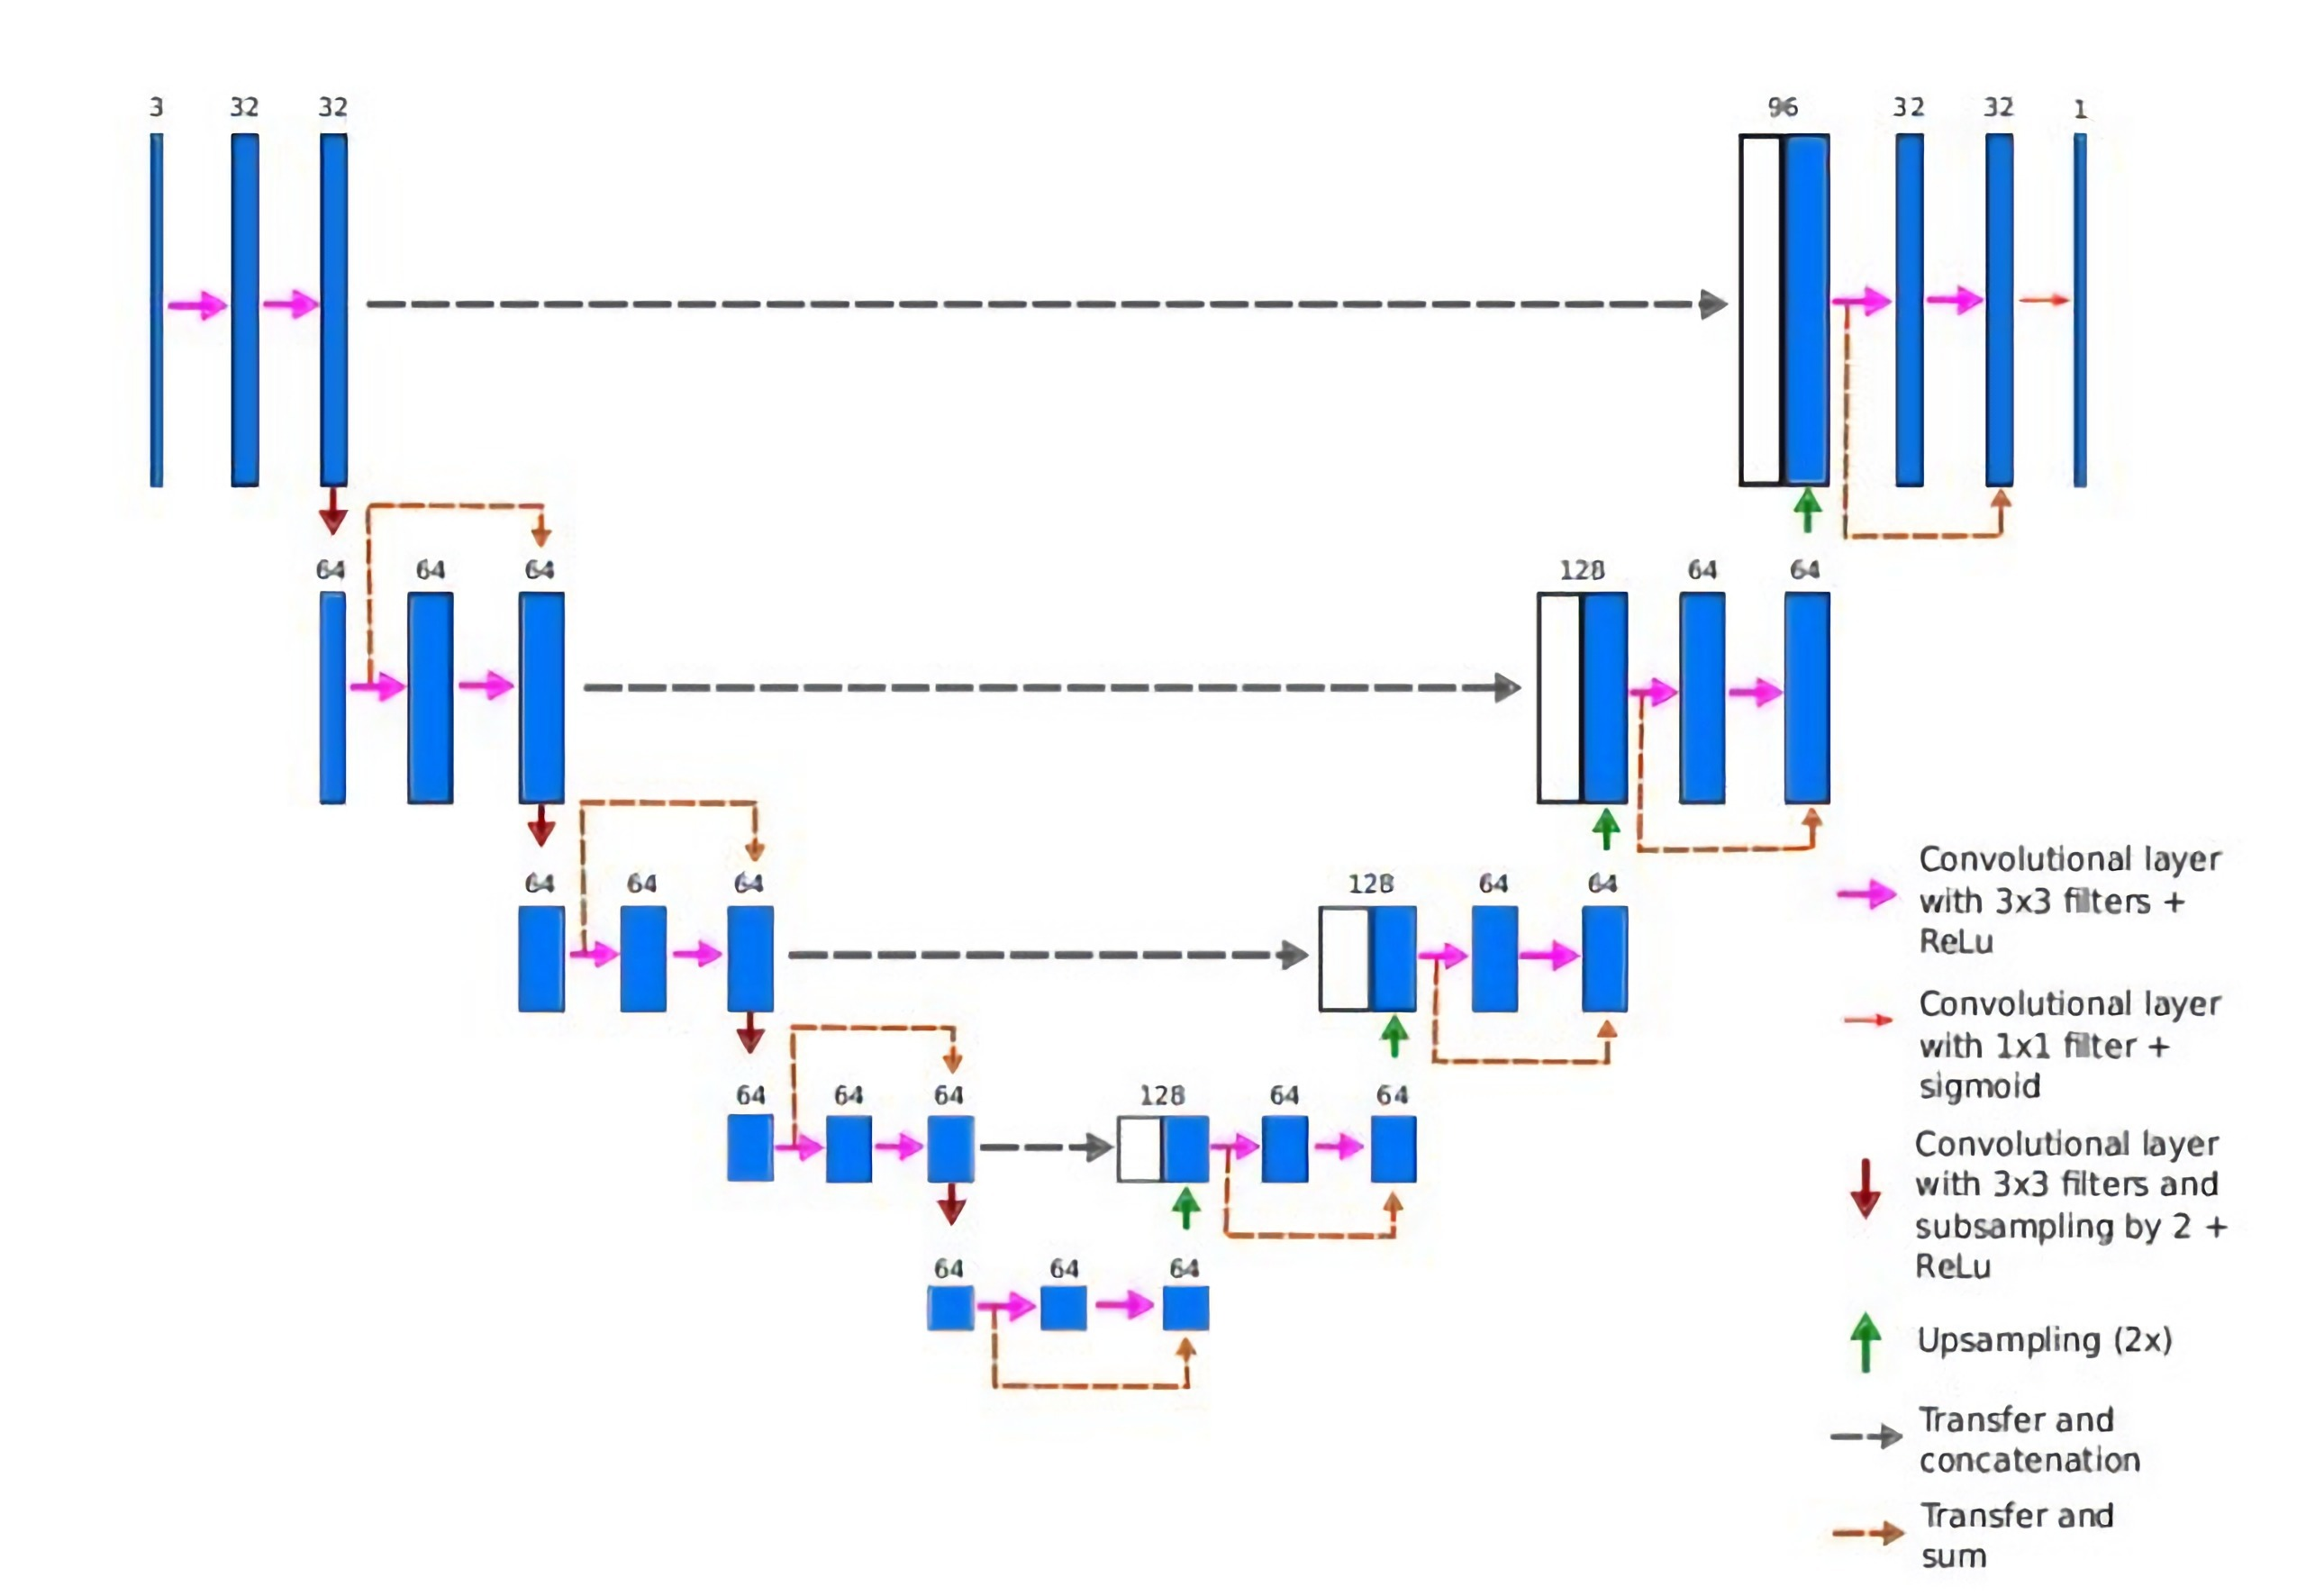
\includegraphics[width=13cm]{Graphics/unet_model.jpg}
    \caption{Arquitectura de una red del tipo U-Net.}
    \label{fig:unet}
\end{figure}